\par\noindent\begin{minipage}{\linewidth}
    \centering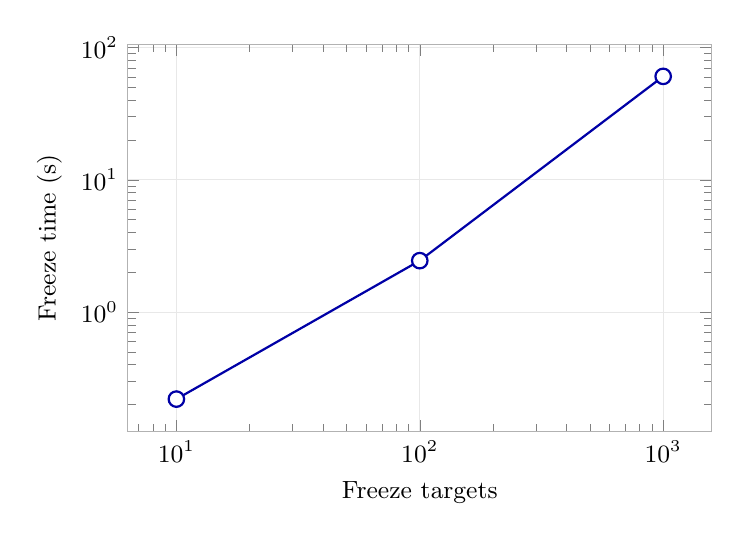
\begin{tikzpicture}
        \begin{axis}[width=9cm,height=6.5cm,grid=major,major grid style={gray!18},axis line style={gray!60},tick label style={font=\small},label style={font=\small},scaled ticks=false,xmode=log,ymode=log,log basis x=10,log basis y=10,xlabel={Freeze targets},ylabel={Freeze time (s)}]
            \addplot+[color=blue!65!black,mark=*,mark size=2.8pt,mark options={solid,fill=white,draw=blue!65!black},thick] coordinates {(10,0.219802208) (100,2.448003417) (1000,60.539842)};
        \end{axis}
    \end{tikzpicture}
    \par\smallskip{\small 그림 3. 동결 대상 수에 따른 Freeze 시간.}\par\medskip
    \par\medskip\noindent
    \begin{center}
        {\small\setlength{\tabcolsep}{7pt}\renewcommand{\arraystretch}{1.12}
            \textbf{Freeze}\par\smallskip
            \begin{tabular}{@{}lr@{}}\toprule
                \textbf{동결 대상 수} & \textbf{시간 (s)} \\
                \midrule
                10               & 0.220           \\
                100              & 2.448           \\
                1,000            & 60.540          \\
                \bottomrule\end{tabular}}
    \end{center}
    \par\medskip
\end{minipage}\par\medskip
